% schem_gate: the factor that one reliability estimate contributes to the
% correction, for the plug-in correction and for Algorithm 1 (gated
% disattenuation), at N=50, K=3, alpha=0.1. Column figure, 3.30 x 1.92 in,
% drawn at final size and included at 100%.
% Build: pdflatex -interaction=nonstopmode -halt-on-error schem_gate.tex
%
% Coordinates are inches from the bottom-left corner.
%   X(r) = 0.42 + (r + 0.50) * 1.85333   for rhat in [-0.50, 1.00]
%   Y(f) = 0.70 + (f - 0.75) * 0.407547  for the factor f in [0.75, 3.40]
% Position-only constants (never printed): qgate = 1.357, qucb = 1.392
% (upper-0.1 quantiles of F(49,100) and F(100,49)), r_g = 1 - 1/qgate = 0.2631,
% L = 1 - 1/(qgate qucb) = 0.4707, 1/sqrt(L) = 1.4575, 1/L = 2.124.
% The gate fails when MSB/MSW <= qgate, so the Algorithm 1 branch is the open
% interval r_g < rhat <= 1 and its factor stays below 1/sqrt(L): the marker at
% the gate is open. The bounding box is inset by the 0.5pt border, so the page
% is exactly 3.30 x 1.92 in.
\documentclass[border=0.5pt]{standalone}
\usepackage{newtxtext,newtxmath}
\usepackage{amsmath}
\usepackage{xcolor}
\usepackage{tikz}
\usetikzlibrary{arrows.meta}

% Macros copied from the paper's LaTeX macro file
\newcommand{\rhat}{\hat{\rho}}
\newcommand{\robs}{r_{\mathrm{obs}}}
\newcommand{\qgate}{q_{\mathrm{gate}}}
\newcommand{\qucb}{q_{\mathrm{ucb}}}
\newcommand{\ICC}[1]{\mathrm{ICC}(#1)}
\newcommand{\clip}{\mathrm{clip}}
\newcommand{\Declined}{\textsc{declined}}

% Palette (figscripts/style.py)
\definecolor{alg}{HTML}{0072B2}
\definecolor{plug}{HTML}{D55E00}
\definecolor{ref}{HTML}{999999}
\definecolor{txt}{HTML}{000000}
\definecolor{txt2}{HTML}{555555}
\definecolor{fillc}{HTML}{F2F2F2}
\definecolor{dens}{HTML}{D9D9D9}

\tikzset{
  t/.style={inner sep=0pt, outer sep=0pt, anchor=base west,
            font=\fontsize{7}{8.4}\selectfont, text=txt},
  tc/.style={t, anchor=base},
  tr/.style={t, anchor=base east},
  ttl/.style={t, font=\fontsize{8}{9.6}\selectfont},
  dashedp/.style={dash pattern=on 2pt off 1.5pt},
  dottedp/.style={dash pattern=on 0.6pt off 1.2pt},
  tip/.style={-{Stealth[length=3pt,width=2.4pt]}},
}

\begin{document}
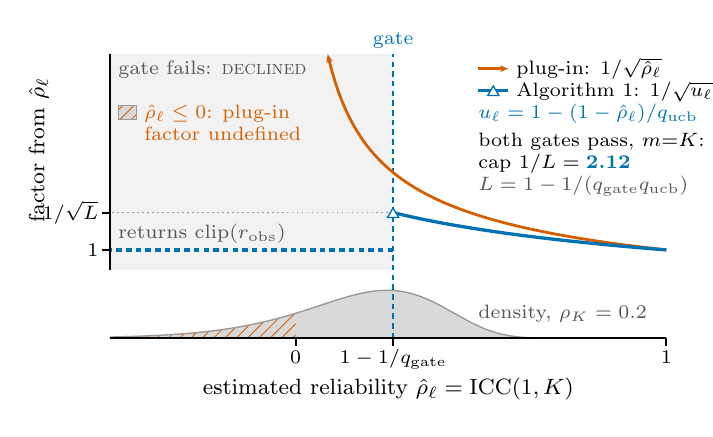
\begin{tikzpicture}[x=1in, y=1in, line width=0.6pt, line cap=butt, line join=miter]
\useasboundingbox (0.5pt,0.5pt) rectangle ([shift={(-0.5pt,-0.5pt)}]3.30,1.92);

% (1) Declined band: left of the gate
\fill[fillc] (0.42,0.70) rectangle (1.834,1.78);

% (2) Density strip: rhat = 1 - (1 - rho_K) F, F ~ F(100,49), rho_K = 0.2,
% 301 points of scipy.stats.f.pdf((1-r)/0.8, 100, 49)/0.8 on r in [-0.50, 1.00],
% scaled so that the peak (r = 0.247) is 0.24 in above the baseline.
\path[save path=\densarea] (0.42,0.36) -- plot coordinates {
  (0.4200,0.3663) (0.4293,0.3665) (0.4385,0.3667) (0.4478,0.3669) (0.4571,0.3671) (0.4663,0.3674) (0.4756,0.3676) (0.4849,0.3679)
  (0.4941,0.3682) (0.5034,0.3684) (0.5127,0.3687) (0.5219,0.3690) (0.5312,0.3693) (0.5405,0.3696) (0.5497,0.3700) (0.5590,0.3703)
  (0.5683,0.3707) (0.5775,0.3710) (0.5868,0.3714) (0.5961,0.3718) (0.6053,0.3722) (0.6146,0.3726) (0.6239,0.3730) (0.6331,0.3734)
  (0.6424,0.3739) (0.6517,0.3743) (0.6609,0.3748) (0.6702,0.3753) (0.6795,0.3758) (0.6887,0.3763) (0.6980,0.3768) (0.7073,0.3774)
  (0.7165,0.3780) (0.7258,0.3786) (0.7351,0.3792) (0.7443,0.3798) (0.7536,0.3804) (0.7629,0.3811) (0.7721,0.3818) (0.7814,0.3825)
  (0.7907,0.3832) (0.7999,0.3840) (0.8092,0.3847) (0.8185,0.3855) (0.8277,0.3863) (0.8370,0.3872) (0.8463,0.3880) (0.8555,0.3889)
  (0.8648,0.3898) (0.8741,0.3908) (0.8833,0.3917) (0.8926,0.3927) (0.9019,0.3938) (0.9111,0.3948) (0.9204,0.3959) (0.9297,0.3970)
  (0.9389,0.3981) (0.9482,0.3993) (0.9575,0.4005) (0.9667,0.4017) (0.9760,0.4030) (0.9853,0.4043) (0.9945,0.4056) (1.0038,0.4070)
  (1.0131,0.4084) (1.0223,0.4098) (1.0316,0.4113) (1.0409,0.4128) (1.0501,0.4144) (1.0594,0.4159) (1.0687,0.4176) (1.0779,0.4192)
  (1.0872,0.4209) (1.0965,0.4227) (1.1057,0.4244) (1.1150,0.4263) (1.1243,0.4281) (1.1335,0.4300) (1.1428,0.4320) (1.1521,0.4340)
  (1.1613,0.4360) (1.1706,0.4381) (1.1799,0.4402) (1.1891,0.4423) (1.1984,0.4445) (1.2077,0.4467) (1.2169,0.4490) (1.2262,0.4513)
  (1.2355,0.4537) (1.2447,0.4561) (1.2540,0.4585) (1.2633,0.4610) (1.2725,0.4635) (1.2818,0.4661) (1.2911,0.4687) (1.3003,0.4713)
  (1.3096,0.4740) (1.3189,0.4767) (1.3281,0.4795) (1.3374,0.4823) (1.3467,0.4851) (1.3559,0.4879) (1.3652,0.4908) (1.3745,0.4937)
  (1.3837,0.4966) (1.3930,0.4996) (1.4023,0.5025) (1.4115,0.5055) (1.4208,0.5085) (1.4301,0.5115) (1.4393,0.5146) (1.4486,0.5176)
  (1.4579,0.5207) (1.4671,0.5237) (1.4764,0.5268) (1.4857,0.5299) (1.4949,0.5329) (1.5042,0.5359) (1.5135,0.5390) (1.5227,0.5420)
  (1.5320,0.5450) (1.5413,0.5479) (1.5505,0.5509) (1.5598,0.5538) (1.5691,0.5566) (1.5783,0.5594) (1.5876,0.5622) (1.5969,0.5649)
  (1.6061,0.5676) (1.6154,0.5702) (1.6247,0.5727) (1.6339,0.5751) (1.6432,0.5775) (1.6525,0.5798) (1.6617,0.5820) (1.6710,0.5841)
  (1.6803,0.5860) (1.6895,0.5879) (1.6988,0.5897) (1.7081,0.5913) (1.7173,0.5929) (1.7266,0.5942) (1.7359,0.5955) (1.7451,0.5966)
  (1.7544,0.5976) (1.7637,0.5984) (1.7729,0.5990) (1.7822,0.5995) (1.7915,0.5998) (1.8007,0.6000) (1.8100,0.6000) (1.8193,0.5998)
  (1.8285,0.5994) (1.8378,0.5988) (1.8471,0.5980) (1.8563,0.5971) (1.8656,0.5959) (1.8749,0.5946) (1.8841,0.5930) (1.8934,0.5913)
  (1.9027,0.5893) (1.9119,0.5872) (1.9212,0.5849) (1.9305,0.5823) (1.9397,0.5796) (1.9490,0.5767) (1.9583,0.5736) (1.9675,0.5703)
  (1.9768,0.5669) (1.9861,0.5633) (1.9953,0.5595) (2.0046,0.5555) (2.0139,0.5514) (2.0231,0.5471) (2.0324,0.5428) (2.0417,0.5382)
  (2.0509,0.5336) (2.0602,0.5288) (2.0695,0.5240) (2.0787,0.5190) (2.0880,0.5140) (2.0973,0.5089) (2.1065,0.5038) (2.1158,0.4986)
  (2.1251,0.4934) (2.1343,0.4881) (2.1436,0.4829) (2.1529,0.4777) (2.1621,0.4725) (2.1714,0.4673) (2.1807,0.4622) (2.1899,0.4571)
  (2.1992,0.4521) (2.2085,0.4471) (2.2177,0.4423) (2.2270,0.4375) (2.2363,0.4329) (2.2455,0.4284) (2.2548,0.4240) (2.2641,0.4198)
  (2.2733,0.4157) (2.2826,0.4117) (2.2919,0.4079) (2.3011,0.4043) (2.3104,0.4008) (2.3197,0.3975) (2.3289,0.3943) (2.3382,0.3914)
  (2.3475,0.3886) (2.3567,0.3859) (2.3660,0.3834) (2.3753,0.3811) (2.3845,0.3790) (2.3938,0.3770) (2.4031,0.3751) (2.4123,0.3735)
  (2.4216,0.3719) (2.4309,0.3705) (2.4401,0.3692) (2.4494,0.3680) (2.4587,0.3670) (2.4679,0.3660) (2.4772,0.3652) (2.4865,0.3645)
  (2.4957,0.3638) (2.5050,0.3632) (2.5143,0.3627) (2.5235,0.3623) (2.5328,0.3619) (2.5421,0.3616) (2.5513,0.3613) (2.5606,0.3611)
  (2.5699,0.3609) (2.5791,0.3607) (2.5884,0.3606) (2.5977,0.3604) (2.6069,0.3603) (2.6162,0.3603) (2.6255,0.3602) (2.6347,0.3602)
  (2.6440,0.3601) (2.6533,0.3601) (2.6625,0.3601) (2.6718,0.3601) (2.6811,0.3600) (2.6903,0.3600) (2.6996,0.3600) (2.7089,0.3600)
  (2.7181,0.3600) (2.7274,0.3600) (2.7367,0.3600) (2.7459,0.3600) (2.7552,0.3600) (2.7645,0.3600) (2.7737,0.3600) (2.7830,0.3600)
  (2.7923,0.3600) (2.8015,0.3600) (2.8108,0.3600) (2.8201,0.3600) (2.8293,0.3600) (2.8386,0.3600) (2.8479,0.3600) (2.8571,0.3600)
  (2.8664,0.3600) (2.8757,0.3600) (2.8849,0.3600) (2.8942,0.3600) (2.9035,0.3600) (2.9127,0.3600) (2.9220,0.3600) (2.9313,0.3600)
  (2.9405,0.3600) (2.9498,0.3600) (2.9591,0.3600) (2.9683,0.3600) (2.9776,0.3600) (2.9869,0.3600) (2.9961,0.3600) (3.0054,0.3600)
  (3.0147,0.3600) (3.0239,0.3600) (3.0332,0.3600) (3.0425,0.3600) (3.0517,0.3600) (3.0610,0.3600) (3.0703,0.3600) (3.0795,0.3600)
  (3.0888,0.3600) (3.0981,0.3600) (3.1073,0.3600) (3.1166,0.3600) (3.1259,0.3600) (3.1351,0.3600) (3.1444,0.3600) (3.1537,0.3600)
  (3.1629,0.3600) (3.1722,0.3600) (3.1815,0.3600) (3.1907,0.3600) (3.2000,0.3600)
} -- cycle;
\fill[dens, use path=\densarea];
% hatching over rhat <= 0, where the plug-in is undefined
\begin{scope}
  \clip (0.42,0.36) -- plot coordinates {
  (0.4200,0.3663) (0.4293,0.3665) (0.4385,0.3667) (0.4478,0.3669) (0.4571,0.3671) (0.4663,0.3674) (0.4756,0.3676) (0.4849,0.3679)
  (0.4941,0.3682) (0.5034,0.3684) (0.5127,0.3687) (0.5219,0.3690) (0.5312,0.3693) (0.5405,0.3696) (0.5497,0.3700) (0.5590,0.3703)
  (0.5683,0.3707) (0.5775,0.3710) (0.5868,0.3714) (0.5961,0.3718) (0.6053,0.3722) (0.6146,0.3726) (0.6239,0.3730) (0.6331,0.3734)
  (0.6424,0.3739) (0.6517,0.3743) (0.6609,0.3748) (0.6702,0.3753) (0.6795,0.3758) (0.6887,0.3763) (0.6980,0.3768) (0.7073,0.3774)
  (0.7165,0.3780) (0.7258,0.3786) (0.7351,0.3792) (0.7443,0.3798) (0.7536,0.3804) (0.7629,0.3811) (0.7721,0.3818) (0.7814,0.3825)
  (0.7907,0.3832) (0.7999,0.3840) (0.8092,0.3847) (0.8185,0.3855) (0.8277,0.3863) (0.8370,0.3872) (0.8463,0.3880) (0.8555,0.3889)
  (0.8648,0.3898) (0.8741,0.3908) (0.8833,0.3917) (0.8926,0.3927) (0.9019,0.3938) (0.9111,0.3948) (0.9204,0.3959) (0.9297,0.3970)
  (0.9389,0.3981) (0.9482,0.3993) (0.9575,0.4005) (0.9667,0.4017) (0.9760,0.4030) (0.9853,0.4043) (0.9945,0.4056) (1.0038,0.4070)
  (1.0131,0.4084) (1.0223,0.4098) (1.0316,0.4113) (1.0409,0.4128) (1.0501,0.4144) (1.0594,0.4159) (1.0687,0.4176) (1.0779,0.4192)
  (1.0872,0.4209) (1.0965,0.4227) (1.1057,0.4244) (1.1150,0.4263) (1.1243,0.4281) (1.1335,0.4300) (1.1428,0.4320) (1.1521,0.4340)
  (1.1613,0.4360) (1.1706,0.4381) (1.1799,0.4402) (1.1891,0.4423) (1.1984,0.4445) (1.2077,0.4467) (1.2169,0.4490) (1.2262,0.4513)
  (1.2355,0.4537) (1.2447,0.4561) (1.2540,0.4585) (1.2633,0.4610) (1.2725,0.4635) (1.2818,0.4661) (1.2911,0.4687) (1.3003,0.4713)
  (1.3096,0.4740) (1.3189,0.4767) (1.3281,0.4795) (1.3374,0.4823) (1.3467,0.4851)
  } -- (1.3467,0.36) -- cycle;
  \foreach \i in {0,...,21}
    \draw[plug, line width=0.3pt] ({0.20+0.056569*\i},0.36) -- ++(0.30,0.30);
\end{scope}
\draw[ref, line width=0.5pt, line join=round, use path=\densarea];

% (3) Gate at X(r_g): one dashed line over the full height
\draw[alg, dashedp] (1.834,0.36) -- (1.834,1.78);
\node[tc, text=alg] at (1.834,1.83) {gate};

% (4) Declined output clip(r_obs): factor 1
\draw[alg, line width=1.2pt, dashedp] (1.834,0.802) -- (0.42,0.802);

% (5) Tick guide at 1/sqrt(L), neutral grey so that only the dashed level
% reads as an output in the declined band
\draw[ref, line width=0.4pt, dottedp] (1.834,0.988) -- (0.42,0.988);

% (6) Plug-in factor 1/sqrt(r) for r from 0.0865 (f = 3.40) to 1,
% sampled in f = 1/sqrt(r). The curve stops inside the arrow tip, which is
% drawn on the chord from f = 3.30 to f = 3.40, so the line does not show
% through the tip.
\draw[plug, line width=1.0pt, line join=round]
  plot[domain=1:3.35, samples=236, variable=\f]
  ({0.42+(1/(\f*\f)+0.5)*1.85333}, {0.70+(\f-0.75)*0.407547});
\draw[plug, line width=1.0pt, tip] (1.5169,1.7392) -- (1.5070,1.7800);

% (7) Algorithm 1 factor 1/sqrt(u), u = 1 - (1 - r)/qucb, r from r_g to 1
\draw[alg, line width=1.2pt, line join=round]
  plot[domain=0.2631:1, samples=150, variable=\r]
  ({0.42+(\r+0.5)*1.85333}, {0.70+(1/sqrt(1-(1-\r)/1.392)-0.75)*0.407547});
% Algorithm 1 marker at the gate: open triangle, 4pt side (the level
% 1/sqrt(L) is the supremum of the branch and is not attained)
\filldraw[alg, fill=white, line width=0.5pt] (1.834,0.988) ++(0,1.7321pt)
  -- ++(-2pt,-3.4641pt) -- ++(4pt,0) -- cycle;

% Spines and ticks
\draw[txt] (0.42,1.78) -- (0.42,0.70);
\draw[txt] (0.42,0.36) -- (3.20,0.36);
\foreach \y in {0.802,0.988} \draw[txt] (0.42,\y) -- (0.38,\y);
\foreach \x in {1.347,1.834,3.200} \draw[txt] (\x,0.36) -- (\x,0.32);
\node[tr] at (0.36,0.770) {$1$};
\node[tr] at (0.36,0.956) {$1/\sqrt{L}$};
\node[ttl, rotate=90, anchor=base] at (0.09,1.30) {factor from $\rhat_\ell$};
\node[tc] at (1.347,0.235) {$0$};
\node[tc] at (1.834,0.235) {$1-1/\qgate$};
\node[tc] at (3.200,0.235) {$1$};
\node[ttl, anchor=base] at (1.81,0.08) {estimated reliability $\rhat_\ell=\ICC{1,K}$};

% Text in the declined band: header, plug-in key, and the label on the
% declined output level
\node[t, text=txt2] at (0.46,1.68) {gate fails: \Declined};
% key for the hatching of the density strip: same fill, hatch and outline
\begin{scope}
  \clip (0.46,1.455) rectangle (0.55,1.525);
  \fill[dens] (0.46,1.455) rectangle (0.55,1.525);
  \foreach \i in {0,...,2}
    \draw[plug, line width=0.3pt] ({0.4134+0.056569*\i},1.455) -- ++(0.12,0.12);
\end{scope}
\draw[ref, line width=0.3pt] (0.46,1.455) rectangle (0.55,1.525);
\node[t, text=plug] at (0.59,1.46) {$\rhat_\ell\le0$: plug-in};
\node[t, text=plug] at (0.59,1.35) {factor undefined};
\node[t, text=txt2] at (0.46,0.860) {returns $\clip(\robs)$};

% Legend: each sample repeats the glyph on its curve
\draw[plug, line width=1.0pt, tip] (2.26,1.708) -- (2.41,1.708);
\node[t] at (2.45,1.68) {plug-in: $1/\sqrt{\rhat_\ell}$};
\draw[alg, line width=1.2pt] (2.26,1.598) -- (2.41,1.598);
\filldraw[alg, fill=white, line width=0.5pt] (2.335,1.598) ++(0,1.7321pt)
  -- ++(-2pt,-3.4641pt) -- ++(4pt,0) -- cycle;
\node[t] at (2.45,1.57) {Algorithm 1: $1/\sqrt{u_\ell}$};
\node[t, text=alg] at (2.26,1.46) {$u_\ell=1-(1-\rhat_\ell)/\qucb$};
\node[t] at (2.26,1.32) {both gates pass, $m{=}K$:};
\node[t] at (2.26,1.21) {cap $1/L=\text{\textcolor{alg}{\textbf{2.12}}}$};
\node[t, text=txt2] at (2.26,1.10) {$L=1-1/(\qgate\qucb)$};

% Density label
\node[t, text=txt2] at (2.26,0.46) {density, $\rho_K=0.2$};
\end{tikzpicture}
\end{document}
